\section{Self-Signed X.509 Certificate}

The creation of a self-signed X.509 was relatively straightforward based off of the commands provided by the course. Below is a list of steps performed, and evidence captured, of our X.509 certificate.

\noindent We first created our certificate based on Jason's details seen in figure \ref{fig:x509_creation:jason}.

\begin{figure}[hbt!]
	\centering
      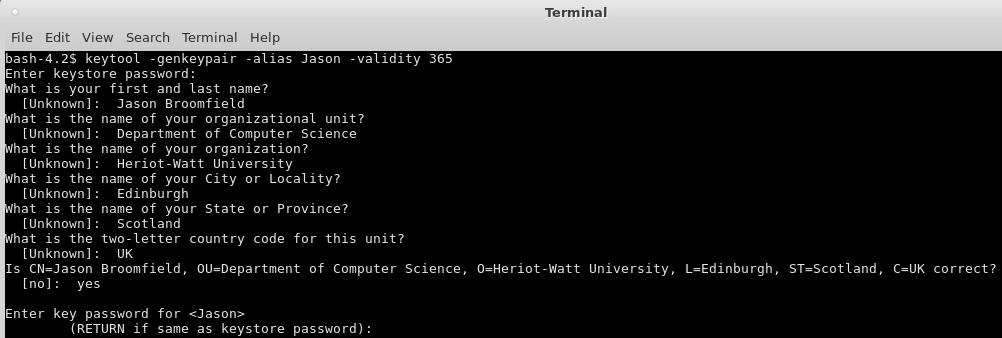
\includegraphics[width=\textwidth]{imgs/x509_creation/x509_creation.PNG} \\
	\caption{Generating X.509 certificate with Jason's details}
	\label{fig:x509_creation:jason}
    \noindent\makebox[\linewidth]{}
\end{figure}

\noindent We then exported the certificate into a \textbf{*.cer} file by the alias name seen in figure \ref{fig:x509_creation:cert_exp}.

\begin{figure}[hbt!]
	\centering
      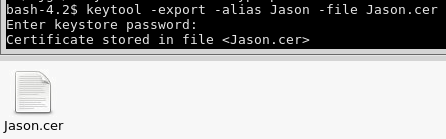
\includegraphics[width=0.5\textwidth]{imgs/x509_creation/x509_certificate_export.PNG} \\
	\caption{Generating X.509 certificate with Jason's details}
	\label{fig:x509_creation:cert_exp}
    \noindent\makebox[\linewidth]{}
\end{figure}

\noindent Viewing the details of the file confirms we have completed this section, as the X.509 file is owned and issued by Jason, displaying a self-signed certificate as seen in figure \ref{fig:x509_creation:cert_exp}.

\begin{figure}[hbt!]
	\centering
      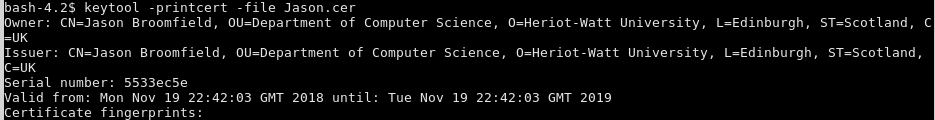
\includegraphics[width=\textwidth]{imgs/x509_creation/cropped.png} \\
	\caption{Generating X.509 certificate with Jason's details}
	\label{fig:x509_creation:cert_deets}
    \noindent\makebox[\linewidth]{}
\end{figure}